%% LyX 2.1.2 created this file.  For more info, see http://www.lyx.org/.
%% Do not edit unless you really know what you are doing.
\documentclass[twocolumn,english,10pt,conference,letterpaper]{RWWTemplate}
\usepackage[T1]{fontenc}
\usepackage{color}
\usepackage{amsmath}
\usepackage{amssymb}
\usepackage{graphicx}

\makeatletter

%%%%%%%%%%%%%%%%%%%%%%%%%%%%%% LyX specific LaTeX commands.
\special{papersize=\the\paperwidth,\the\paperheight}

%% A simple dot to overcome graphicx limitations
\newcommand{\lyxdot}{.}


\makeatother

\usepackage{babel}
\begin{document}

\title{\textcolor{red}{A Closed Form Solution for Frame Slotted ALOHA Utilizing }}


\author{\textcolor{red}{Hazem A. Ahmed, Hamed Salah, Joerg Robert, Albert
Heuberger}\\
\textcolor{red}{Friedrich-Alexander-Universit�t Erlangen-N�rnberg}\\
\textcolor{red}{{} Email: \{hazem.a.elsaid, hamed.kenawy, joerg.robert,
albert.heuberger\}@fau.de}}
\maketitle
\begin{abstract}
\textcolor{red}{Minimizing the reading time of large tag populations
is a critical issue in Radio Frequency Identification (RFID) systems.
The usual approach to reduce the reading time is to select the frame
size attaining the highest throughput per frame. Previous studies
have focused on conventional frame length calculations. In such systems,
only the answer of a single tag is considered as a successful slot.
If multiple tags respond simultaneously within a slot a collision
occurs. Then, all tags within this slot are discarded. However, modern
system have the capability of converting part of the collided slots
into successful slots. This is called Collision Recovery. Moreover,
modern RFID readers have the ability to identify the type of the slot
(successful, collided, or empty). Then, the readers are able to terminate
the slot earlier when they recognizes that there is no tag reply.
This system is called a time aware system. Recent studies focused
on calculating the optimal frame length taking into consideration
the time aware and the collision recovery properties. However, these
studies have assumed constant collision recovery probability coefficients,
i.e. the probability to recover one tag from $i$ collided tags is
constant, regardless of the number of collided tags $i$. Moreover,
they proposed only numerical solutions for the optimum frame length.
In this paper we propose a novel closed form solution for the optimal
Frame Slotted ALOHA (FSA) frame length. The novel solution considers
the multiple collision recovery probability coefficients, and the
different slot durations. Timing comparisons are presented in the
simulation results to show the reading time reduction using the proposed
frame length compared to other the state-of-the-art algorithms.}

\textcolor{red}{\pagenumbering{gobble}}
\end{abstract}


\section{\textcolor{red}{Introduction}}

\textcolor{red}{Radio Frequency Identification (RFID) is an identification
technology that wirelessly transmits the identity of a tag which may
be attached to an object or a person. If tags respond simultaneously
to a reader, a collision on the air interface occurs and the information
is discarded, leading to reduced throughput. Our research focuses
on the improvement of the throughput using the EPCglobal class 1 gen
2 RFID standards \cite{standard}. The conventionally used anti-collision
algorithm is Framed Slotted ALOHA (FSA), which is a Medium Access
Control (MAC) layer protocol. Using this algorithm, only the single
tag replies (successful slot) are able to be decoded and then identified.
Therefore, the conventional definition of the reading efficiency $\eta_{conv}$
is equivalent to the probability of success $P(S)$ \cite{Aloha4_Vogt}:}

\textcolor{red}{\footnotesize{}
\begin{equation}
\eta_{_{conv}}=P(S)=P(1),\label{eq:eff basic equ}
\end{equation}
}\textcolor{red}{where, }\textcolor{red}{\footnotesize{}$P(1)=\frac{n}{L}\left(1-\frac{1}{L}\right)^{n-1}$}\textcolor{red}{,
$n$ represents the number of tags in the reading area, and $L$ is
the frame length. }

\textcolor{red}{The main goal is to find the optimal frame length
$L$, which maximizes the reading efficiency $\eta_{conv}$. Based
on (\ref{eq:eff basic equ}), the reading efficiency $\eta_{_{conv}}$
is maximized to $\eta_{_{conv(max)}}=36\%$ when $L=n$ \cite{Aloha4_Vogt}.
\cite{2012_journal_CR} considered the RFID reader capability of collision
resolving. They have used the characteristics of the RFID signals
to separate signals from collisions on the physical layer (PHY). They
have proposed a new reading efficiency metric that includes the tags
which are recovered based on the PHY layer. The authors assumed that
the probability to recover a single tag from $i$ collided tags is
constant and equals to $100\%$, independently of the value of $i$.
However in reality, the probability to recover a single tag from $i$
collided tags reduces with the number of collided tags $i$. Moreover,
there are no practical readers that offer a $100\%$ collision recovery
probability. Finally, the authors did not consider the effects of
the different slot durations. In \cite{CR_TA_2015}, the authors merged
the collision recovery probability with the effect of the different
slut durations for a new reading efficiency metric. They have assumed
also a constant collision recovery capability, regardless of the number
of collided tags. However, this probability decreases with an increasing
number of collided tags. Moreover, they proposed a numerical solution
for the optimum frame length by searching for the value of the frame
length $L$ which maximizes the reading efficiency. Thus, they require
a Multi-dimensional look-up table.}

\textcolor{red}{In this paper, we propose a novel reading efficiency
metric called Time Aware Multiple Collision Recovery Coefficients
Reading Efficiency $\eta_{_{TAMCRC}}$. The new metric includes different
collision recovery coefficients for each number of collided tags.
Furthermore, it takes into consideration the different slot durations.
Hence, we propose a novel closed form solution for the optimum FSA
frame length at RFID systems. The proposed solution gives a direct
relation between the optimal frame length and the number of tags $n$
in the reading area, in addition to the collision recovery coefficients
and the different slot durations.}

\textcolor{red}{This paper organized as follows: Section II presents
the system model under variable slot duration and multiple collision
recovery coefficients and the proposed corresponding closed form solution
for the optimal frame length. Then, section III gives numerical results
on the improvements of the new optimization criterion, before we conclude
in section IV. }


\section{\textcolor{red}{Proposed System Model }}

\textcolor{red}{In this section we present a new FSA reading efficiency
metric called Time Aware Multiple Collision Recovery Coefficients
Reading Efficiency $\eta_{_{TAMCRC}}$. The main contribution in this
new efficiency is: It contains a unique collision recovery coefficient
$\alpha_{i}$ for each probability of collision $P(i)$. These new
coefficients indicate the ability of the reader to recover one tag
from $i$ collided tags, where this ability varies based on the number
of collided tags. Moreover, it takes into consideration the different
slot durations. }

\textcolor{red}{Figure \ref{fig:Collision-distribution-in} presents
the distribution of the average collision probability in a frame length
uniformly distributed within }\textcolor{red}{\scriptsize{}$0.5\leq\frac{L}{n}\leq2$}\textcolor{red}{,
which is the practical range of the RFID frame length. According to
figure \ref{fig:Collision-distribution-in}, the probability that
a collision results from two or three collided tags is approx. $85\%$.
Moreover, the values of the collision recovery coefficient $\alpha_{i}$
when $i\geq4$ (i\@.e\@. 4 or more collided tags) will be small.
Therefore, we will only consider up to three collided tags. We will
now normalize the slot duration $t_{k}$ of successful and collided
tags to unity. We furthermore take the assumption that empty slots
are shorter than successful slots (i\@.e\@. $t_{0}\leq t_{k}$),
which is the case for practical readers. Then, the proposed reading
efficiency $\eta_{_{TAMCRC}}$ can be expressed as:}

\textcolor{red}{\scriptsize{}
\begin{equation}
\eta_{_{TAMCRC}}=\frac{P(1)+\alpha_{2}P_{col.}(2)+\alpha_{3}P_{col.}(3)}{1+P(0)\cdot(C_{t}-1)},\label{eq:new coll prob}
\end{equation}
}\textcolor{red}{where $C_{t}=\frac{t_{0}}{t_{k}}$ represents the
slots duration constant, and $\alpha_{2}$, $\alpha_{3}$ are respectively
the second, third collision recovery coefficients. }
\begin{figure}
\textcolor{red}{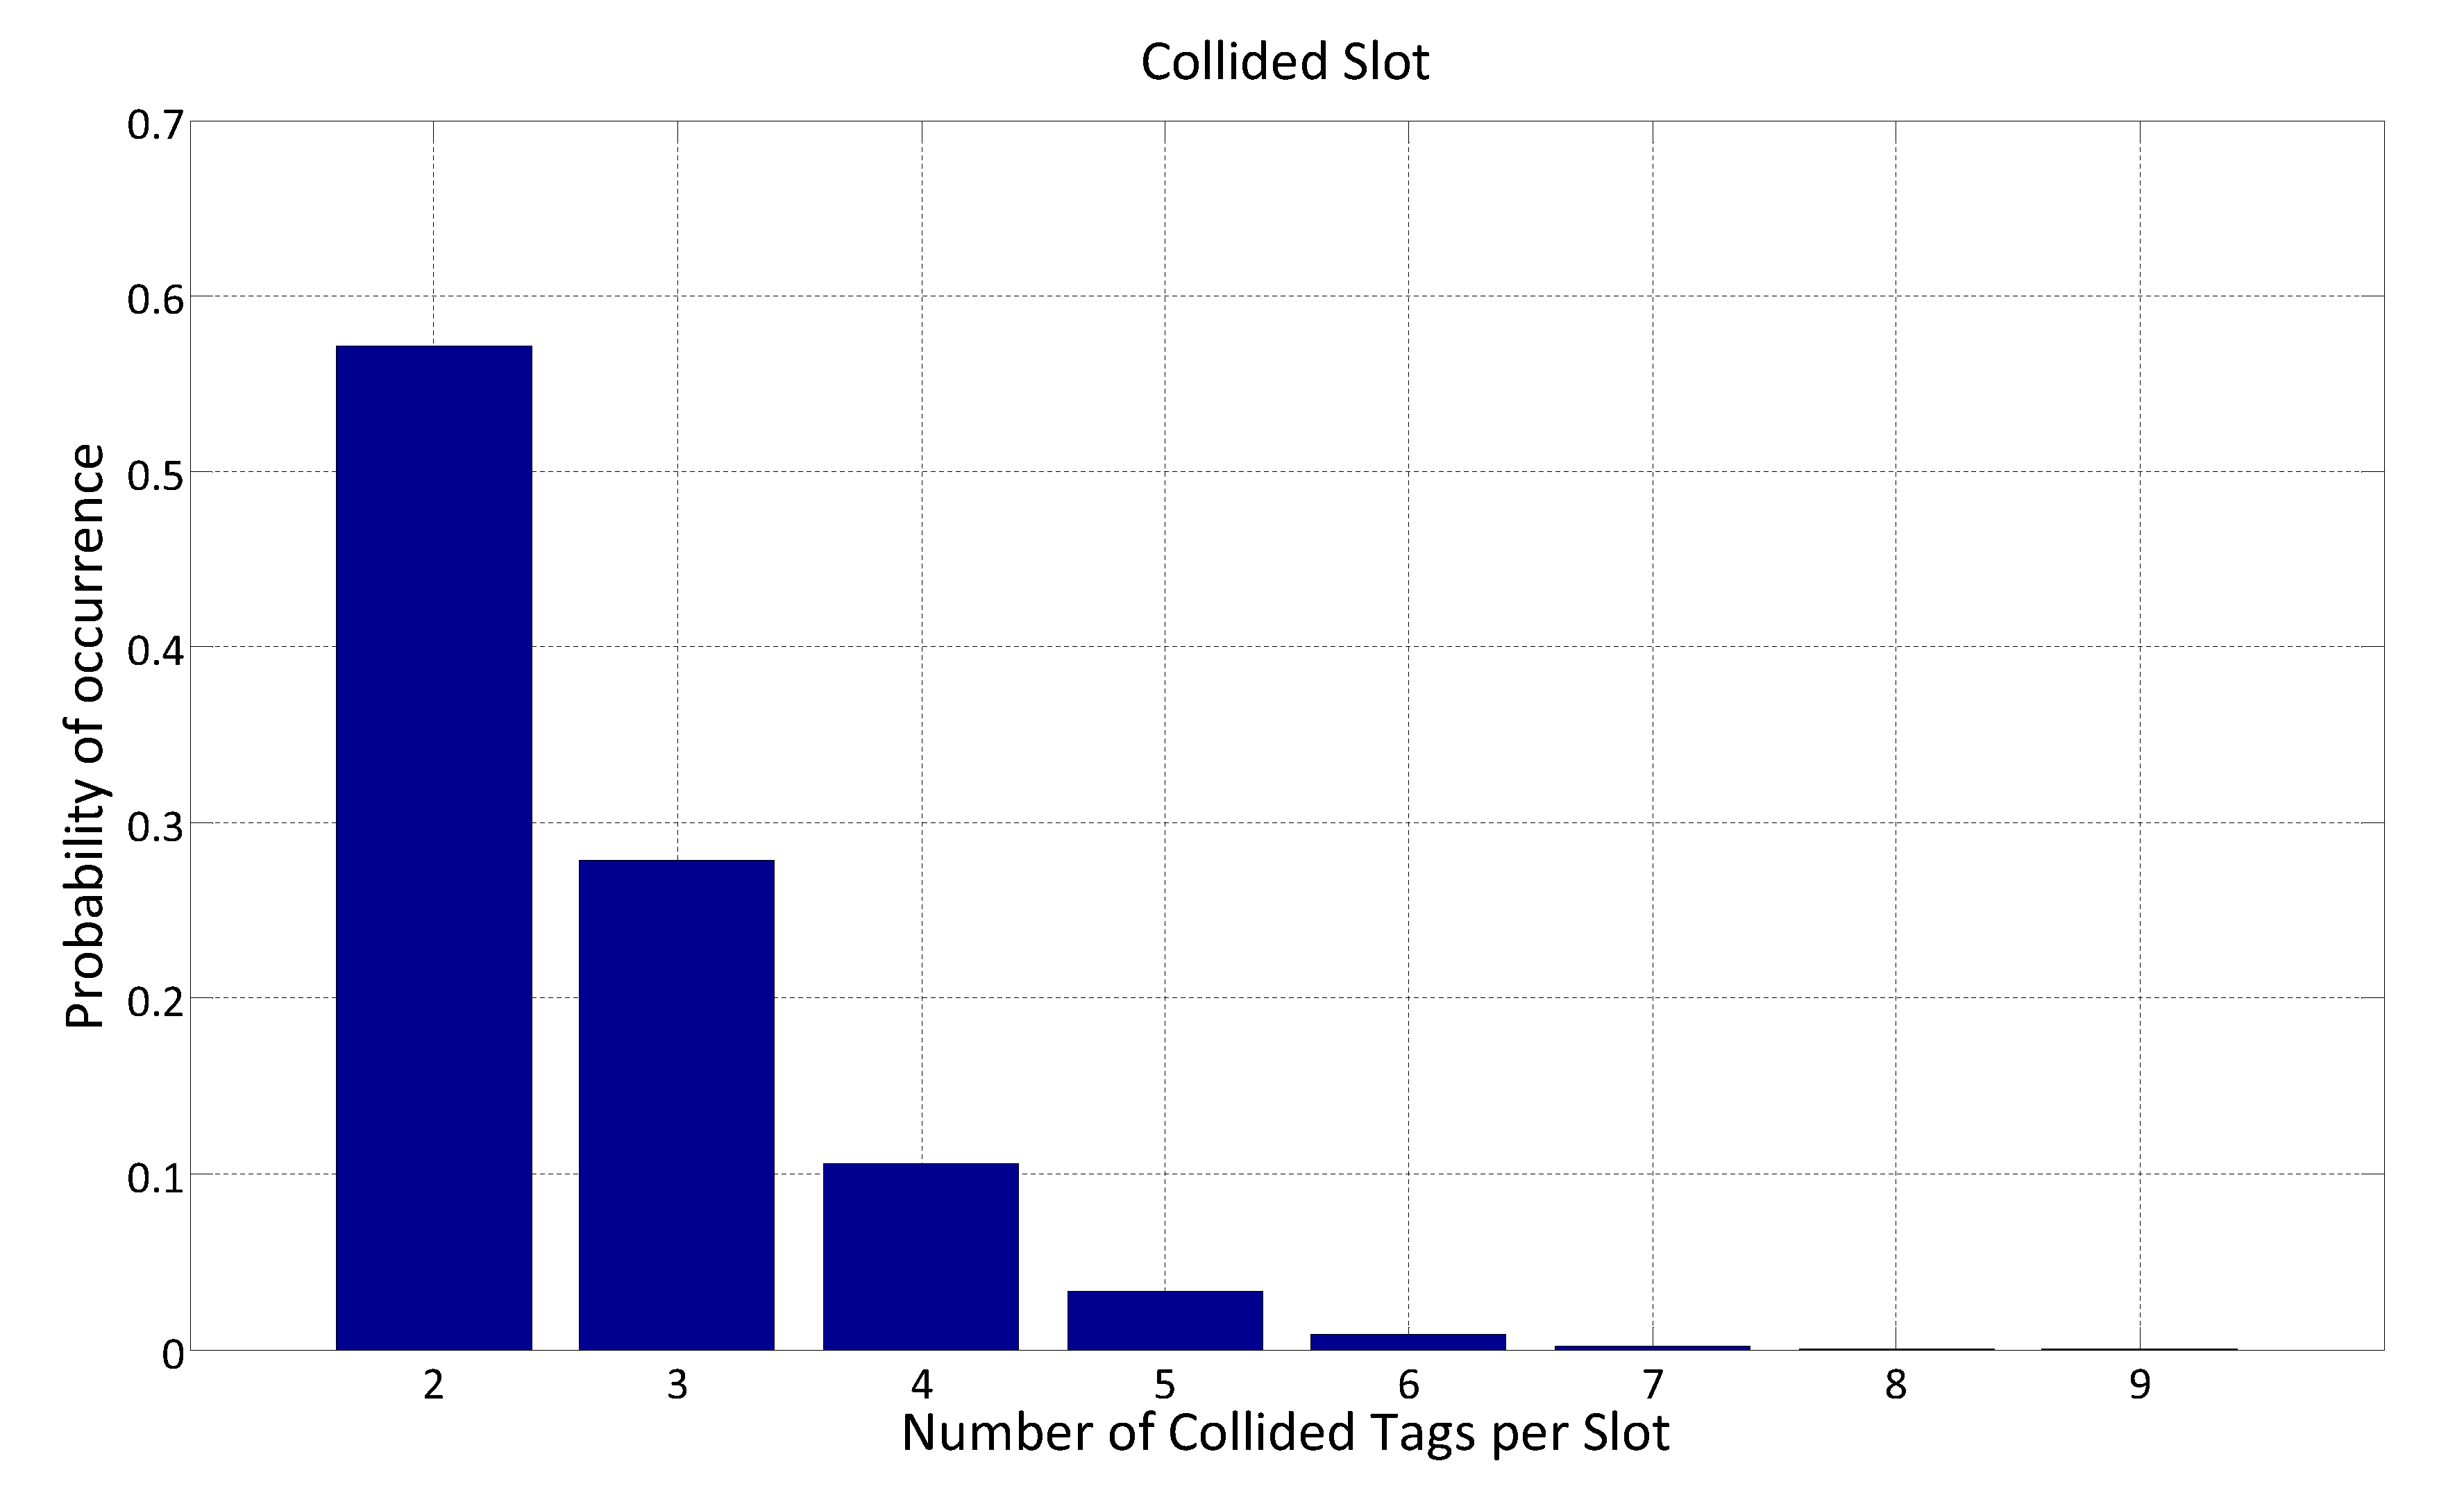
\includegraphics[width=1\columnwidth]{collision_distribution}}

\textcolor{red}{\protect\caption{Collision distribution probability in FSA, under condition of $\frac{n}{2}\leq L\leq2n$
\label{fig:Collision-distribution-in}}
}
\end{figure}


\textcolor{red}{The next step is to derive a closed form for the new
optimum frame length $L_{_{TAMCRC}}$ which maximizes $\eta_{_{TAMCRC}}$.
According to \cite{2013_orthogonal}, if $L\gg1$, and $n\gg i$ we
get:}

\textcolor{red}{\scriptsize{}
\begin{equation}
P(i)\backsimeq\frac{1}{i!}\cdot\beta^{-i}\cdot e^{-\frac{1}{\beta}},\label{eq:approx_P(i)}
\end{equation}
}\textcolor{red}{where, $\beta=\frac{L}{n}$. After substituting by
(\ref{eq:approx_P(i)}) in (\ref{eq:new coll prob}) we obtain:}

\textcolor{red}{\scriptsize{}
\begin{equation}
\eta_{_{TAMCRC}}=\frac{e^{-\frac{1}{\beta}}\cdot\left(\beta^{-1}+\frac{\alpha_{2}}{2}\beta^{-2}+\frac{\alpha_{3}}{6}\beta^{-3}\right)}{1+e^{-\frac{1}{\beta}}\cdot(C_{t}-1)}\label{eq:eff_proposed_simpl}
\end{equation}
}\textcolor{red}{Now we have to find the value of $\beta$ which maximizes
$\eta_{_{TAMCRC}}$. This is achieved by differentiating the reading
efficiency in (\ref{eq:eff_proposed_simpl}) with respect to $\beta$
and equate the result to zero:}

\textcolor{red}{\scriptsize{}
\begin{equation}
\frac{\partial\eta_{_{TAMCRC}}}{\partial\beta}=0\label{eq:diff}
\end{equation}
}\textcolor{red}{After differentiating and simplifications, the final
equation is a fourth order polynomial:}

\textcolor{red}{\footnotesize{}
\begin{equation}
a\cdot\beta^{4}+b\cdot\beta^{3}+c\cdot\beta^{2}+d\cdot\beta+e=0,\label{eq:final_fourth}
\end{equation}
}\textcolor{red}{where: }\textcolor{red}{\scriptsize{}$a=\underset{(-)}{\underbrace{-C_{t}}}$,
$b=\underset{(-)}{\underbrace{C_{t}\cdot(1-\alpha_{2})-1}}$}{\scriptsize \par}

\textcolor{red}{\scriptsize{}$c=\underset{(+)}{\underbrace{\underset{(+)}{\underbrace{2-C_{t}-\alpha_{2}}}+\underset{(+)}{\underbrace{\frac{C_{t}}{2}(\alpha_{2}-\alpha_{3})}}}}$}{\scriptsize \par}

\textcolor{red}{\scriptsize{}$d=\underset{(+)}{\underbrace{\frac{1}{2}(\alpha_{2}-\alpha_{3})+\frac{1}{2}\alpha_{2}\cdot(1-C_{t})+\frac{1}{6}C_{t}\cdot\alpha_{3}}}$}{\scriptsize \par}

\textcolor{red}{\scriptsize{}$e=\underset{(+)}{\underbrace{\frac{1}{6}\alpha_{3}\cdot(2-C_{t})}}$}\\
\textcolor{red}{As $0\leq\alpha_{i}\leq1$, $0<C_{t}\leq1$, and $\alpha_{2}\geq\alpha_{3}$,
equation (\ref{eq:final_fourth}) has four roots \cite{Math_book_quartic}:}

\textcolor{red}{\scriptsize{}
\begin{eqnarray}
\beta_{1,2} & = & -\frac{b}{4a}-S\pm0.5\sqrt{\underset{X}{\underbrace{-4S^{2}-2P+\frac{q}{S}}}}\label{eq:roots}\\
\beta_{3,4} & = & -\frac{b}{4a}+S\pm0.5\sqrt{\underset{Y}{\underbrace{-4S^{2}-2P-\frac{q}{S}}}},\nonumber 
\end{eqnarray}
}\textcolor{red}{with $P=\frac{8ac-3b^{2}}{8a^{2}}$, $q=\frac{b^{3}-4abc+8a^{2}d}{8a^{3}}$}\\
\textcolor{red}{and}\textcolor{red}{\scriptsize{} $S=0.5\sqrt{-\frac{2}{3}P+\frac{1}{3a}\left(Q+\frac{\triangle_{0}}{Q}\right)}$,~~~~$Q=\sqrt[3]{\frac{\triangle_{1}+\sqrt{\triangle_{1}^{2}-4\triangle_{0}^{3}}}{2}}$}\textcolor{red}{}\\
\textcolor{red}{}\\
\textcolor{red}{with}\textcolor{red}{\scriptsize{} $\triangle_{0}=c^{2}-3bd+12ae$,~~~~~~$\triangle_{1}=2c^{3}-9bcd+27ad^{2}-72ace$}{\scriptsize \par}

\textcolor{red}{According to the practical ranges of the collision
recovery coefficients $\alpha_{i}$ and $C_{t}$, we can prove that
the signs of the polynomial coefficients are constants and do not
change in all ranges of $\alpha_{i}$ and $C_{t}.$ Thus their signs
will be: }\\
\textcolor{red}{$a=(-)$, $b=(-)$, $c=(+)$, $d=(+)$, and $e=(+)$.}\\
\textcolor{red}{Using Descartes\textquoteright{} rules of sign \cite{Descartes_rule}
we can count the number of real positive solutions of the polynomial.}

\textcolor{red}{Let us assume that the polynomial in (\ref{eq:final_fourth})
is $P(\beta)$, and let $\nu$ be the number of variations in the
sign of the coefficients $a,\, b,\, c,\, d,\, e$, i\@.e\@. $\nu=1$,
and let $n_{p}$ be the number of real positive solutions. According
to Descartes\textquoteright{} rules of sign \cite{Descartes_rule}
we get:}
\begin{itemize}
\item \textcolor{red}{$n_{p}\leq\nu$, which means that $n_{p}=0\,\textrm{or}\,1$.}
\item \textcolor{red}{$\nu-n_{p}$ is an even integer. Therefore $n_{p}=1$.}
\end{itemize}
\textcolor{red}{Consequently, there is only one valid real positive
solution, one valid real negative solution, and two complex solutions
for our equation. Our target is to identify which solution from the
four solutions is the valid one. We have either $\beta_{1,2}$ or
$\beta_{3,4}$ real solutions, so $S$ should be a positive real number,
and the complex values come only from the square roots $\sqrt{X}$
and $\sqrt{Y}$ . According to the coefficient signs: $q$ must be
always positive real value. Therefore, in (\ref{eq:roots}) the value
of $X>Y$. So $\beta_{3,4}$ have to be the complex roots, with $\beta_{1}>\beta_{2}$.
Therefore, $\beta_{2}$ is the negative root and $\beta_{1}$ is the
positive real root. Based on the above discussions, the proposed closed
form optimum frame length $L_{TAMCRC}$ under time and multiple collision
recovery coefficients environment leads to:}

\textcolor{red}{\scriptsize{}
\begin{equation}
L_{TAMCRC}=\left(-\frac{b}{4a}-S+0.5\sqrt{-4S^{2}-2P+\frac{q}{S}}\right)\cdot n\label{eq:closed form}
\end{equation}
}\textcolor{red}{The proposed equation gives a linear relation wrt.
the number of tags $n$, and includes the effect of different collision
recovery coefficients and the slot duration constant. The values of
these coefficients are set based on the RFID reader type as shown
in \cite{2012_orthogonal_codes}. The value of $C_{t}$ can be calculated
based on the transmission rate as shown in \cite{Ct_calculation}.
Based on (\ref{eq:closed form}), if the RFID reader has no collision
resolving capability ($\alpha_{2}=\alpha_{3}=0$) and equal slots
durations are used ($C_{t}=1$), we get $L_{TAMCRC}=n$. This is identical
to the optimum frame length in the conventional case. }
\begin{figure}
\textcolor{red}{\includegraphics[width=1\columnwidth]{Max_eff_validation_0\lyxdot 1_0\lyxdot 5_0\lyxdot 9}}

\textcolor{red}{\protect\caption{Maximum reading efficiency $0\leq C_{t}\leq1$ \label{fig:Maximum-efficiency-using}}
}
\end{figure}



\section{\textcolor{red}{Simulation Results}}

\textcolor{red}{In this section, we will firstly discuss the accuracy
of our closed form, then we will show the gain of using the proposed
closed form shown in (\ref{eq:closed form}) in terms of mean reading
time reduction compared to the literature. Figure \ref{fig:Maximum-efficiency-using}
presents the maximum efficiency using the proposed closed form compared
to the numerical solutions in \cite{CR_TA_2015} for different values
of collision recovery coefficients $\alpha_{i}$ in the full range
of the slots duration constant $C_{t}$. It is clear that the proposed
formula almost approaches the numerical solution. There is a small
bias between the curves due to the approximation in (\ref{eq:approx_P(i)}).
However, the closed form equation has a direct relation of the optimum
frame length function of the number of tags in the reading area, the
collision recovery coefficients, and the slots duration constant,
so we need neither storage nor searching each reading cycle. However
using the numerical methods, we have to store and search in a multidimensional
look-up table to get the optimal frame length corresponding to each
parameters combination.}

\textcolor{red}{Figure \ref{fig:Mean-reduction-in} presents the mean
reading time reduction using the proposed frame length equation compared
to the frame length proposed by \cite{2012_journal_CR}. The simulation
results are based on the slot duration constant $C_{t}=0.2$, as it
is considered as a practical value used in the EPCglobal class 1 gen
2 standards \cite{standard}. The authors in \cite{2012_journal_CR}
used identical collision recovery coefficients, then based on that
has a constant frame lengths. According to figure \ref{fig:Mean-reduction-in},
the mean reduction in reading time increases, when the collision recovery
coefficients decreases. In this case, the proposed frame length will
adapt for the new optimum size. However, the frame length proposed
by \cite{2012_journal_CR} is fixed based on the assumption of $100\%$
collision recovery capability. }


\section{\textcolor{red}{Conclusion}}

\textcolor{red}{This paper proposes a novel closed form solution for
the optimum value of the FSA (Frame Slotted ALOHA) frame length in
RFID systems. The proposed equation takes the effect of different
collision recovery probabilities into account, as well as the different
slot durations. The theoretical derivations lead to a new optimization
criterion that can be easily implemented in RFID readers. The closed
form solution needs neither storage nor searching like the numerical
solutions presented in the literature. Timing comparisons were presented
to show the mean reading time reduction using the proposed frame length
compared to other proposals.}


\section*{\textcolor{red}{Acknowledgment}}

\textcolor{red}{The authors are grateful to department OK at Fraunhofer
IIS in Erlangen, Germany, for the support of this work.}

\textcolor{red}{}
\begin{figure}
\textcolor{red}{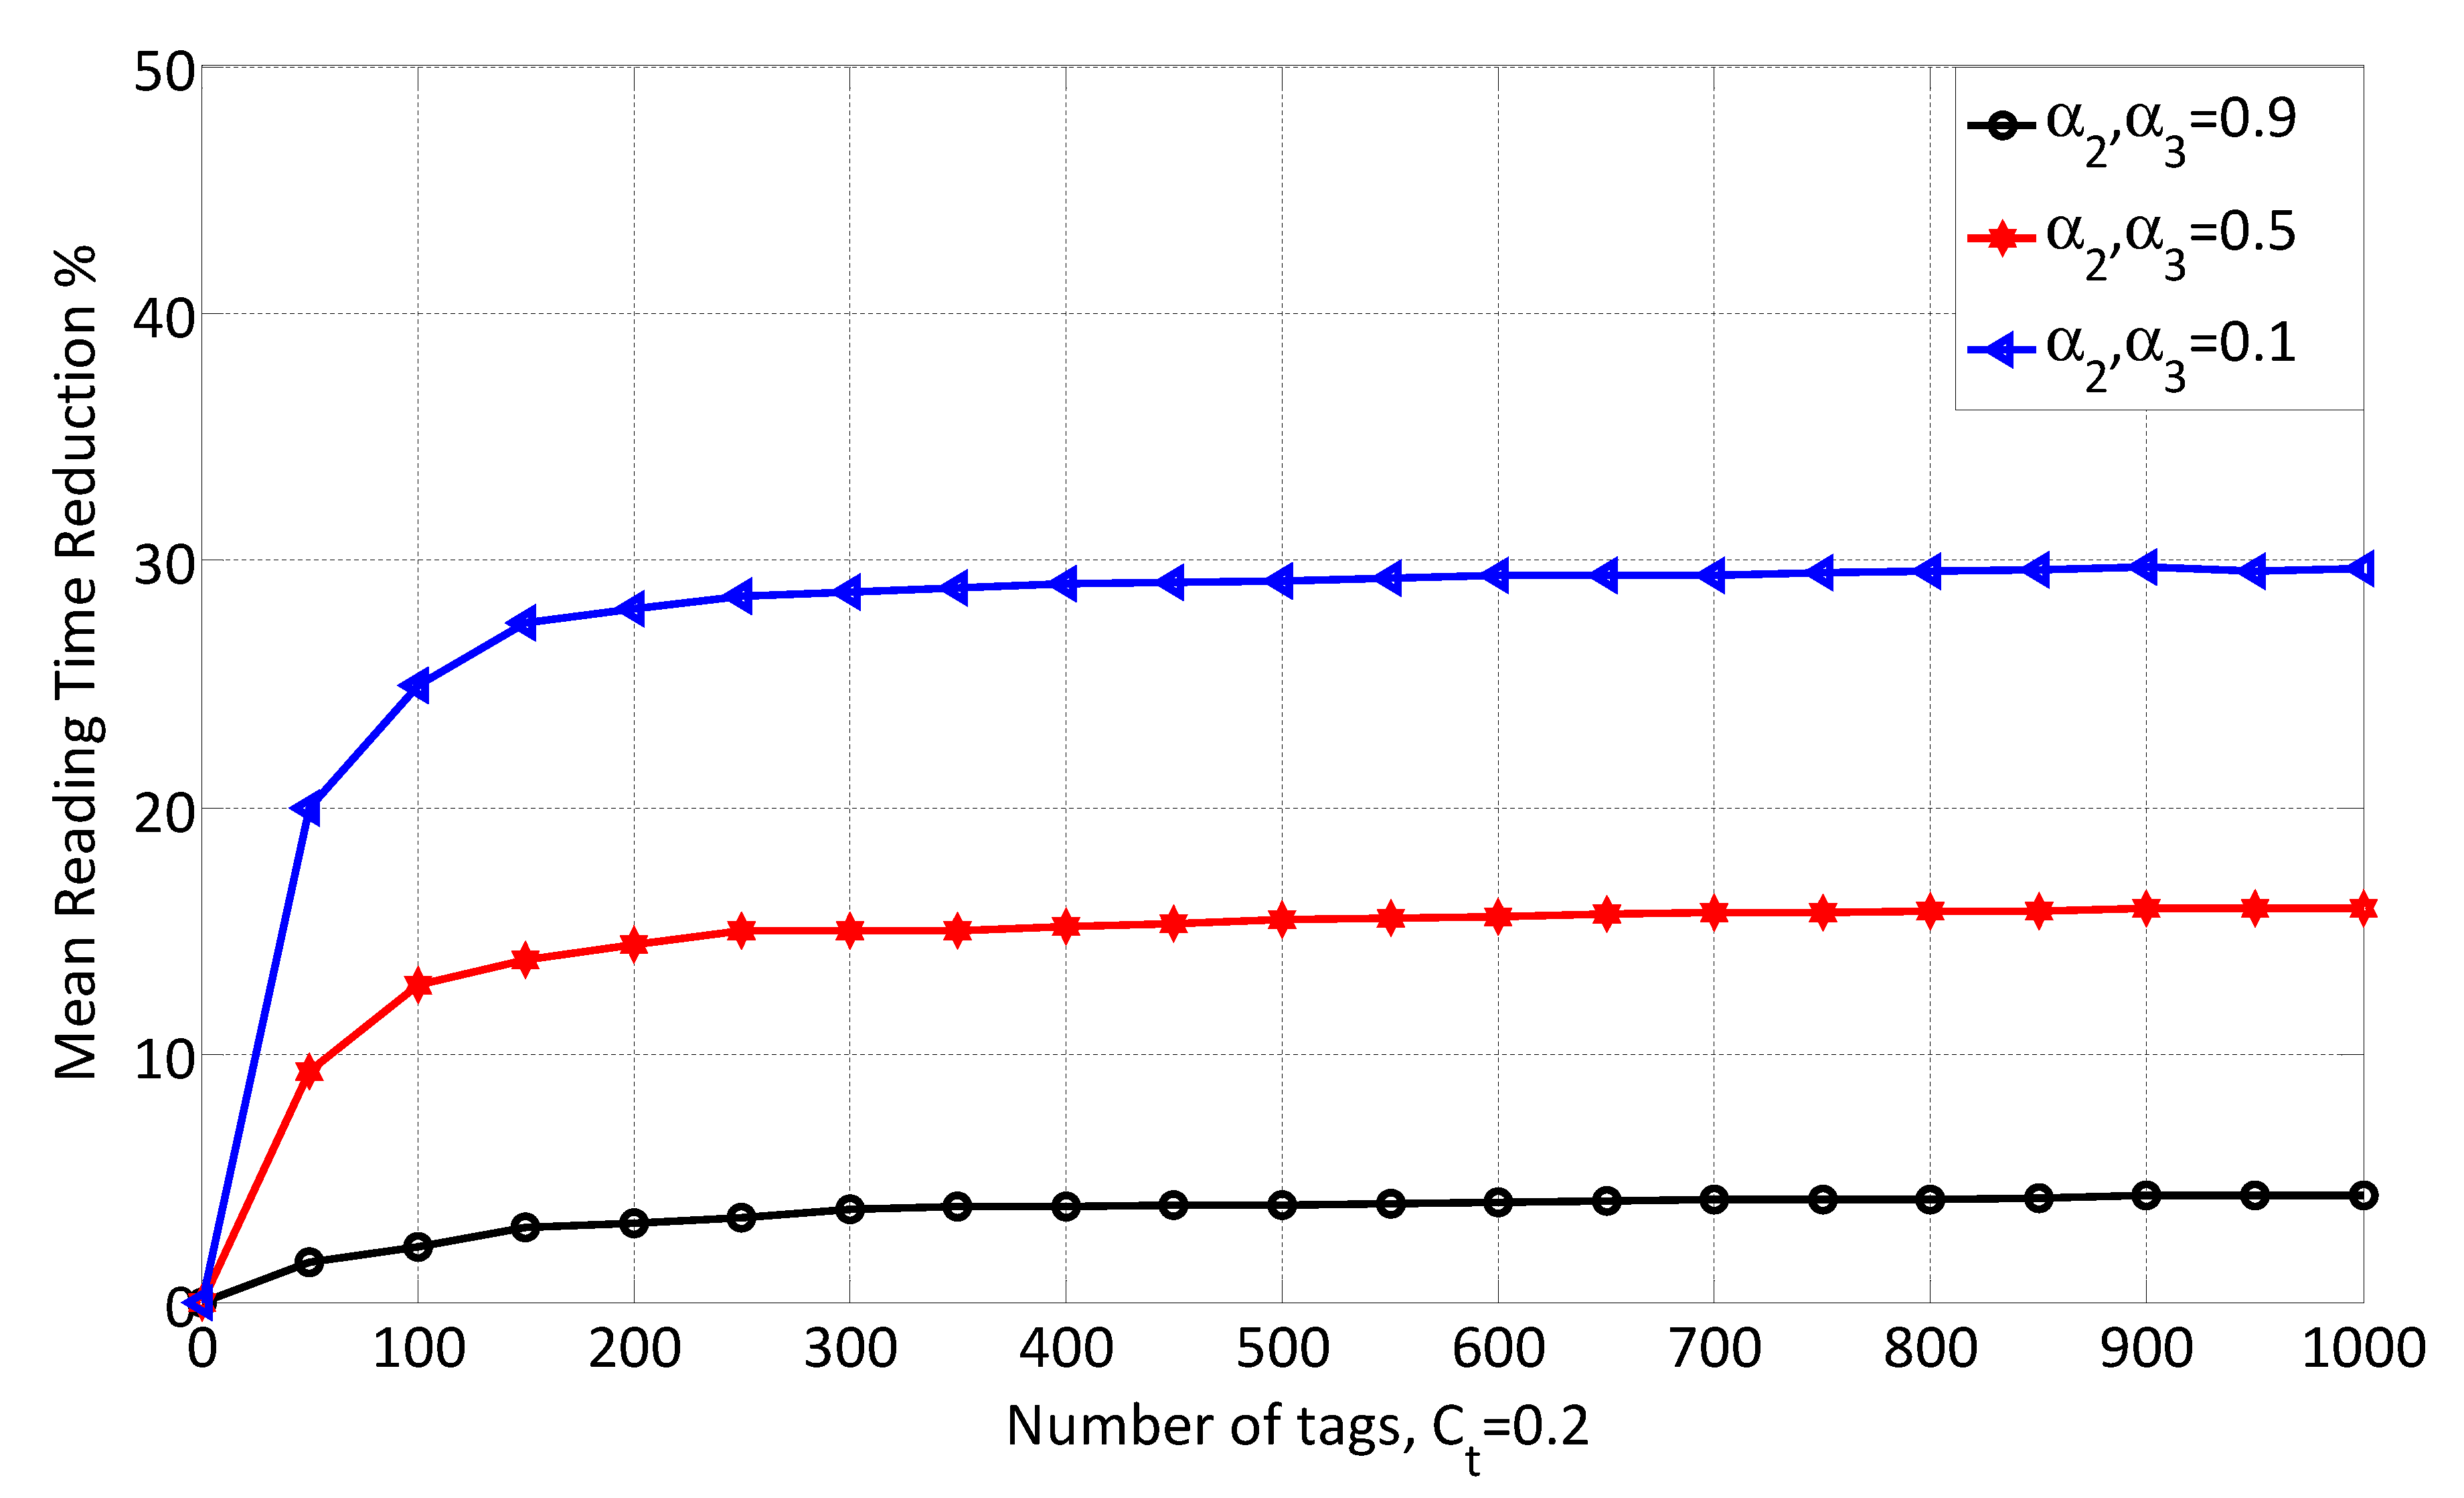
\includegraphics[width=1\columnwidth]{saving_time_new}\protect\caption{Mean reading time reduction using the proposed frame length compared
to the proposal of \cite{2012_journal_CR} \label{fig:Mean-reduction-in}}
}
\end{figure}


\textcolor{red}{\bibliographystyle{ieeetr}
\bibliography{Lopt_PJY_MAC}
}
\end{document}
